% Select document class: uncomment one of the following
\documentclass[aspectratio=169]{beamer}  % For presentation mode
%\documentclass[11pt]{article}            % For article mode
%\usepackage{beamerarticle}               % Uncomment with article class

% =============================================================================
% COMMON PREAMBLE
% =============================================================================
% =============================================================================
% Common Preamble for Network+ Lecture Series
% This file provides consistent formatting, colors, packages, and styles
% across all lecture modules for both beamer presentations and article mode
% =============================================================================

% =============================================================================
% THEME AND COLORS
% =============================================================================
\usetheme{Madrid}
\usecolortheme{whale}

% Custom colors - standardized across all lectures
\definecolor{rctcblue}{RGB}{0, 74, 136}
\definecolor{rctcgold}{RGB}{255, 199, 44}
\definecolor{networkgreen}{RGB}{0, 128, 64}
\definecolor{alertred}{RGB}{180, 0, 0}
\definecolor{aborange}{RGB}{230, 126, 34}
\definecolor{copperbrown}{RGB}{184, 115, 51}
\definecolor{faborange}{RGB}{255, 165, 0}
\definecolor{fiberyellow}{RGB}{255, 215, 0}
\definecolor{shirepurple}{RGB}{102, 51, 153}
\definecolor{ipblue}{RGB}{52, 152, 219}
\definecolor{ippurple}{RGB}{155, 89, 182}
\definecolor{vlangreen}{RGB}{39, 174, 96}
\definecolor{tcpblue}{RGB}{30, 100, 180}
\definecolor{udpgreen}{RGB}{50, 160, 80}
\definecolor{dhcppurple}{RGB}{120, 60, 160}
\definecolor{dnsyellow}{RGB}{200, 170, 50}
\definecolor{batblack}{RGB}{30, 30, 40}
\definecolor{gothamgray}{RGB}{80, 85, 95}
\definecolor{paddysgreen}{RGB}{19, 77, 33}
\definecolor{beerlight}{RGB}{255, 199, 44}
\definecolor{sunnyorange}{RGB}{255, 140, 0}
\definecolor{ogregreen}{RGB}{34, 139, 34}
\definecolor{swampbrown}{RGB}{101, 67, 33}

% Set theme colors
\setbeamercolor{palette primary}{bg=rctcblue,fg=white}
\setbeamercolor{palette secondary}{bg=rctcblue!80,fg=white}
\setbeamercolor{palette tertiary}{bg=rctcblue!60,fg=white}
\setbeamercolor{structure}{fg=rctcblue}
\setbeamercolor{title}{fg=white,bg=rctcblue}
\setbeamercolor{frametitle}{fg=white,bg=rctcblue}
\setbeamercolor{block title}{bg=rctcblue,fg=white}
\setbeamercolor{block body}{bg=rctcblue!10,fg=black}
\setbeamercolor{block title alerted}{bg=alertred,fg=white}
\setbeamercolor{block body alerted}{bg=alertred!10,fg=black}
\setbeamercolor{block title example}{bg=networkgreen,fg=white}
\setbeamercolor{block body example}{bg=networkgreen!10,fg=black}

% =============================================================================
% PACKAGES
% =============================================================================
\usepackage[utf8]{inputenc}
\usepackage[T1]{fontenc}
\usepackage{lmodern}  % Better font rendering
\usepackage{graphicx}
\usepackage{tikz}
\usepackage{booktabs}
\usepackage{array}
\usepackage{multirow}
\usepackage{hyperref}
\usepackage{adjustbox}
\usepackage{amssymb}
\usepackage{amsmath}
\usepackage{calc}
\usepackage{fontawesome5}
% xcolor with [table] option: avoid colortbl.4ht hook conflict in tex4ht
\ifdefined\HCode
  \usepackage{xcolor}
  \usepackage{colortbl}  % provides \rowcolor etc.
\else
  \usepackage[table]{xcolor}  % includes colortbl for pdflatex
\fi

% =============================================================================
% TIKZ LIBRARIES AND SETUP
% =============================================================================
\usetikzlibrary{
    shapes.geometric,
    shapes.symbols,
    shapes.misc,
    arrows.meta,
    positioning,
    calc,
    fit,
    backgrounds,
    decorations.pathreplacing,
    decorations.pathmorphing,
    matrix,
    chains
}
% shadows library causes pgfuseshading errors with tex4ht;
% only load it when NOT building HTML
\ifdefined\HCode\else
    \usetikzlibrary{shadows}
\fi

% Graphics path for icons and chapter images
\graphicspath{
    {../images/icons/}
    {./images/icons/}
    {images/icons/}
    {../images/ch1/}
    {./images/ch1/}
    {images/ch1/}
    {../images/ch2/}
    {./images/ch2/}
    {images/ch2/}
    {../images/ch3/}
    {./images/ch3/}
    {images/ch3/}
    {../images/ch4/}
    {./images/ch4/}
    {images/ch4/}
    {../images/ch5/}
    {./images/ch5/}
    {images/ch5/}
    {../images/ch6/}
    {./images/ch6/}
    {images/ch6/}
    {../images/ch7/}
    {./images/ch7/}
    {images/ch7/}
    {../images/ch8/}
    {./images/ch8/}
    {images/ch8/}
    {../images/ch9/}
    {./images/ch9/}
    {images/ch9/}
    {../images/}
    {./images/}
    {images/}
}

% =============================================================================
% NETWORK DIAGRAM STYLES
% =============================================================================
\tikzset{
    % Node styles for network devices
    device/.style={
        inner sep=2pt,
        label distance=2pt
    },
    pc/.style={device},
    laptop/.style={device},
    server/.style={device},
    router/.style={device},
    switch/.style={device},
    firewall/.style={device},
    cloud/.style={device},
    phone/.style={device},
    tablet/.style={device},
    wifi/.style={device},
    % Connection styles
    ethernet/.style={
        draw=rctcblue,
        line width=1.5pt,
        -{Stealth[length=3mm]}
    },
    ethernet noarrow/.style={
        draw=rctcblue,
        line width=1.5pt
    },
    wireless/.style={
        draw=aborange,
        line width=1.5pt,
        dashed,
        -{Stealth[length=3mm]}
    },
    wireless noarrow/.style={
        draw=aborange,
        line width=1.5pt,
        dashed
    },
    wan/.style={
        draw=alertred,
        line width=2pt,
        -{Stealth[length=3mm]}
    },
    wan noarrow/.style={
        draw=alertred,
        line width=2pt
    },
    copper/.style={
        draw=copperbrown,
        line width=2pt,
        -{Stealth[length=3mm]}
    },
    copper noarrow/.style={
        draw=copperbrown,
        line width=2pt
    },
    fiber/.style={
        draw=fiberyellow,
        line width=2pt,
        -{Stealth[length=3mm]}
    },
    fiber noarrow/.style={
        draw=fiberyellow,
        line width=2pt
    },
    trunk/.style={
        draw=shirepurple,
        line width=2pt,
        -{Stealth[length=3mm]}
    },
    trunk noarrow/.style={
        draw=shirepurple,
        line width=2pt
    },
    % Packet/segment styles
    pktseg/.style={
        draw=rctcblue,
        fill=rctcblue!10,
        minimum height=0.5cm,
        font=\tiny,
        rounded corners=2pt
    },
    pktseg tcp/.style={
        draw=tcpblue,
        fill=tcpblue!15,
        minimum height=0.5cm,
        font=\tiny,
        rounded corners=2pt
    },
    pktseg udp/.style={
        draw=udpgreen,
        fill=udpgreen!15,
        minimum height=0.5cm,
        font=\tiny,
        rounded corners=2pt
    },
    pktseg highlight/.style={
        draw=aborange,
        fill=aborange!20,
        minimum height=0.5cm,
        font=\tiny,
        rounded corners=2pt
    },
    % Box styles
    ipbox/.style={
        draw=rctcblue,
        fill=rctcblue!10,
        rounded corners,
        minimum height=0.4cm,
        font=\small
    },
    portbox/.style={
        draw=tcpblue,
        fill=tcpblue!10,
        rounded corners,
        minimum height=0.4cm,
        font=\small
    },
    dnsbox/.style={
        draw=dnsyellow,
        fill=dnsyellow!15,
        rounded corners,
        minimum height=0.4cm,
        font=\small
    },
    routetable/.style={
        draw=rctcblue,
        fill=rctcblue!10,
        rounded corners,
        minimum height=0.4cm,
        font=\small
    },
    macbox/.style={
        draw=networkgreen,
        fill=networkgreen!10,
        rounded corners,
        minimum height=0.4cm,
        font=\small
    },
    % Frame segment styles (Ethernet frame diagrams)
    frameseg/.style={
        draw=rctcblue,
        fill=rctcblue!10,
        minimum height=0.5cm,
        font=\tiny,
        rounded corners=2pt
    },
    frameseg highlight/.style={
        draw=aborange,
        fill=aborange!20,
        minimum height=0.5cm,
        font=\tiny,
        rounded corners=2pt
    },
    % Process/flow styles
    process/.style={
        draw=rctcblue,
        fill=rctcblue!15,
        rounded corners,
        minimum width=2cm,
        minimum height=0.6cm,
        font=\small,
        align=center
    },
    decision/.style={
        draw=aborange,
        fill=aborange!15,
        diamond,
        aspect=2,
        minimum width=1.5cm,
        font=\small,
        align=center
    },
    % OSI Layer styles
    osilayer/.style={
        draw=rctcblue,
        fill=rctcblue!10,
        minimum width=3cm,
        minimum height=0.45cm,
        font=\small
    },
    osilayer highlight/.style={
        draw=aborange,
        fill=aborange!20,
        line width=1.5pt,
        minimum width=3cm,
        minimum height=0.45cm,
        font=\small\bfseries
    }
}

% =============================================================================
% ICON COMMANDS - Standardized using PNG files and FontAwesome
% =============================================================================
% Network device icons (PNG)
\newcommand{\iconpc}[1][0.6cm]{\resizebox{#1}{!}{
\includegraphics{icon_pc}}}
\newcommand{\iconlaptop}[1][0.6cm]{\resizebox{#1}{!}{
\includegraphics{icon_laptop}}}
\newcommand{\iconserver}[1][0.6cm]{\resizebox{#1}{!}{
\includegraphics{icon_server}}}
\newcommand{\iconrouter}[1][0.6cm]{\resizebox{#1}{!}{
\includegraphics{icon_router}}}
\newcommand{\iconswitch}[1][0.6cm]{\resizebox{#1}{!}{
\includegraphics{icon_switch}}}
\newcommand{\iconfirewall}[1][0.6cm]{\resizebox{#1}{!}{
\includegraphics{icon_firewall}}}
\newcommand{\iconcloud}[1][0.6cm]{\resizebox{#1}{!}{
\includegraphics{icon_cloud}}}
\newcommand{\iconphone}[1][0.6cm]{\resizebox{#1}{!}{
\includegraphics{icon_phone}}}
\newcommand{\icontablet}[1][0.6cm]{\resizebox{#1}{!}{
\includegraphics{icon_tablet}}}
\newcommand{\iconwifi}[1][0.6cm]{\resizebox{#1}{!}{
\includegraphics{icon_wifi}}}
\newcommand{\icondatabase}[1][0.6cm]{\resizebox{#1}{!}{
\includegraphics{icon_db}}}
\newcommand{\iconlock}[1][0.6cm]{\resizebox{#1}{!}{
\includegraphics{icon_lock}}}

% For HTML/tex4ht builds: replace PNG icons with FontAwesome5 glyphs.
% dvisvgm embeds font glyphs as vectors but silently ignores em:graph (PNG)
% specials, so PNG icons would be blank in the output SVGs. FA5 glyphs work.
\ifdefined\HCode
  \renewcommand{\iconpc}[1][0.6cm]{\resizebox{#1}{!}{\faIcon{desktop}}}
  \renewcommand{\iconlaptop}[1][0.6cm]{\resizebox{#1}{!}{\faIcon{laptop}}}
  \renewcommand{\iconserver}[1][0.6cm]{\resizebox{#1}{!}{\faIcon{server}}}
  \renewcommand{\iconrouter}[1][0.6cm]{\resizebox{#1}{!}{\faIcon{route}}}
  \renewcommand{\iconswitch}[1][0.6cm]{\resizebox{#1}{!}{\faIcon{network-wired}}}
  \renewcommand{\iconfirewall}[1][0.6cm]{\resizebox{#1}{!}{\faIcon{shield-alt}}}
  \renewcommand{\iconcloud}[1][0.6cm]{\resizebox{#1}{!}{\faIcon{cloud}}}
  \renewcommand{\iconphone}[1][0.6cm]{\resizebox{#1}{!}{\faIcon{mobile-alt}}}
  \renewcommand{\icontablet}[1][0.6cm]{\resizebox{#1}{!}{\faIcon{tablet-alt}}}
  \renewcommand{\iconwifi}[1][0.6cm]{\resizebox{#1}{!}{\faIcon{wifi}}}
  \renewcommand{\icondatabase}[1][0.6cm]{\resizebox{#1}{!}{\faIcon{database}}}
  \renewcommand{\iconlock}[1][0.6cm]{\resizebox{#1}{!}{\faIcon{lock}}}
\fi

% FontAwesome icons
\newcommand{\iconuser}[1][0.6cm]{\resizebox{#1}{!}{\faIcon{user}}}
\newcommand{\iconglobe}[1][0.6cm]{\resizebox{#1}{!}{\faIcon{globe}}}
\newcommand{\iconclock}[1][0.6cm]{\resizebox{#1}{!}{\faIcon{clock}}}
\newcommand{\iconmail}[1][0.6cm]{\resizebox{#1}{!}{\faIcon{envelope}}}
\newcommand{\icondoc}[1][0.6cm]{\resizebox{#1}{!}{\faIcon{file-alt}}}
\newcommand{\iconsearch}[1][0.6cm]{\resizebox{#1}{!}{\faIcon{search}}}
\newcommand{\icontools}[1][0.6cm]{\resizebox{#1}{!}{\faIcon{tools}}}
\newcommand{\iconchart}[1][0.6cm]{\resizebox{#1}{!}{\faIcon{chart-line}}}
\newcommand{\iconalert}[1][0.6cm]{\resizebox{#1}{!}{\faIcon{bell}}}
\newcommand{\iconlog}[1][0.6cm]{\resizebox{#1}{!}{\faIcon{clipboard-list}}}
\newcommand{\iconeye}[1][0.6cm]{\resizebox{#1}{!}{\faIcon{eye}}}
\newcommand{\iconhacker}[1][0.6cm]{\resizebox{#1}{!}{\faIcon{user-secret}}}
\newcommand{\iconkey}[1][0.6cm]{\resizebox{#1}{!}{\faIcon{key}}}
\newcommand{\iconfile}[1][0.6cm]{\resizebox{#1}{!}{\faIcon{file-alt}}}
\newcommand{\icondog}[1][0.6cm]{\resizebox{#1}{!}{\faIcon{dog}}}
\newcommand{\iconcat}[1][0.6cm]{\resizebox{#1}{!}{\faIcon{cat}}}
\newcommand{\iconvoip}[1][0.6cm]{\resizebox{#1}{!}{\faIcon{phone-volume}}}
\newcommand{\iconmoney}[1][0.6cm]{\resizebox{#1}{!}{\faIcon{money-bill-wave}}}
\newcommand{\icontrash}[1][0.6cm]{\resizebox{#1}{!}{\faIcon{trash}}}
\newcommand{\iconbuilding}[1][0.6cm]{\resizebox{#1}{!}{\faIcon{building}}}

% =============================================================================
% CUSTOM COMMANDS AND ENVIRONMENTS
% =============================================================================

% Key term formatting
\newcommand{\keyterm}[1]{\textbf{#1}}

% Slide section marker
\newcommand{\sectionslide}[1]{
    \begin{frame}
        \vfill
        \centering
        \begin{beamercolorbox}[sep=8pt,center,shadow=true,rounded=true]{title}
            \usebeamerfont{title}\Huge #1
        \end{beamercolorbox}
        \vfill
    \end{frame}
}

% Case study frame environment
\newenvironment{casestudy}[1]{%
    \begin{alertblock}{$\blacktriangleright$ Case Study: #1}
}{%
    \end{alertblock}
}

% Solution frame environment  
\newenvironment{casesolution}[1]{%
    \begin{exampleblock}{$\checkmark$ Solution: #1}
}{%
    \end{exampleblock}
}

% =============================================================================
% FOOTER WITH SLIDE NUMBERS
% =============================================================================
\setbeamertemplate{footline}{
    \leavevmode%
    \hbox{%
        \begin{beamercolorbox}[wd=.333333\paperwidth,ht=2.25ex,dp=1ex,center]{author in head/foot}%
            \usebeamerfont{author in head/foot}\insertshortauthor
        \end{beamercolorbox}%
        \begin{beamercolorbox}[wd=.333333\paperwidth,ht=2.25ex,dp=1ex,center]{title in head/foot}%
            \usebeamerfont{title in head/foot}\insertshorttitle
        \end{beamercolorbox}%
        \begin{beamercolorbox}[wd=.333333\paperwidth,ht=2.25ex,dp=1ex,right]{date in head/foot}%
            \usebeamerfont{date in head/foot}\insertshortdate{}\hspace*{2em}
            \insertframenumber{} / \inserttotalframenumber\hspace*{2ex}
        \end{beamercolorbox}}%
    \vskip0pt%
}

% =============================================================================
% ARTICLE MODE SUPPORT
% =============================================================================
% The following commands help with beamerarticle mode for HTML conversion

% In article mode, add proper section/subsection support and override environments
\mode<article>{
    % Make sure figure captions work properly
    \setbeamertemplate{caption}[numbered]
    \setbeamertemplate{caption label separator}{: }
    
    % Add some spacing for readability
    \setlength{\parskip}{0.5em}
    \setlength{\parindent}{0pt}
    
    % Article mode versions of case study environments
    \renewenvironment{casestudy}[1]{%
        \vspace{0.3cm}\noindent\textbf{Case Study: #1}\newline\begin{itshape}
    }{%
        \end{itshape}\vspace{0.3cm}
    }
    
    \renewenvironment{casesolution}[1]{%
        \vspace{0.3cm}\noindent\textbf{Solution: #1}\newline\begin{itshape}
    }{%
        \end{itshape}\vspace{0.3cm}
    }
}

% Command to mark content that only appears in article mode
\newcommand{\articleonly}[1]{\mode<article>{#1}}

% Command to mark content that only appears in presentation mode
\newcommand{\presentationonly}[1]{\mode<presentation>{#1}}


% =============================================================================
% DOCUMENT INFO
% =============================================================================
\title[Identity and Hardening]{Module 10: Identity, Access, and Network Hardening}
\subtitle{Intro to Networks}
\author{Brendan Shea, PhD}
\institute{Rochester Community and Technical College}
\date{}

\begin{document}

% =============================================================================
% Module 10: Identity, Access, and Network Hardening
% =============================================================================

\begin{frame}
    \titlepage
    \begin{center}
        \begin{tikzpicture}[scale=0.8]
            \node (id) at (-2.8, 0) {\faIcon{id-badge}};
            \node[below=0.1cm of id, font=\tiny] {Identity};
            \node (shield) at (0, 0) {\faIcon{shield-alt}};
            \node[below=0.1cm of shield, font=\tiny] {Hardening};
            \node (sw) at (2.8, 0) {\iconswitch[0.9cm]};
            \node[below=0.1cm of sw, font=\tiny] {Policy Enforcement};
            \draw[->, thick, rctcblue] (id) -- (shield);
            \draw[->, thick, networkgreen] (shield) -- (sw);
        \end{tikzpicture}
    \end{center}
\end{frame}

\presentationonly{
\begin{frame}[allowframebreaks]{Outline}
\small
\tableofcontents[hideallsubsections]
\end{frame}
}

% =============================================================================
\section*{Review from Module 9}
% =============================================================================

\begin{frame}{Review: Security Concepts Foundations}
    \begin{columns}[T]
        \begin{column}{0.48\textwidth}
            \begin{block}{Key Module 9 Ideas}
                \begin{itemize}
                    \item The \textbf{CIA triad}: Confidentiality (keep secrets), Integrity (prevent tampering), Availability (keep systems running).
                    \item Threats include malware, phishing, spoofing, and denial-of-service attacks.
                    \item Defense in depth layers multiple controls so no single failure causes total compromise.
                \end{itemize}
            \end{block}
        \end{column}
        \begin{column}{0.48\textwidth}
            \begin{alertblock}{Where Module 10 Takes This}
                Module 9 described the \emph{threats}. Module 10 gives us the \emph{tools to fight back}: controlling who gets in, what they are allowed to do, and how we lock systems down.
            \end{alertblock}
        \end{column}
    \end{columns}
\end{frame}

% =============================================================================
\section*{Learning Outcomes}
% =============================================================================

\begin{frame}[t,allowframebreaks]{Learning Outcomes}
    After completing this module, you will be able to:
    \vspace{0.5em}
    \small
    \begin{itemize}
        \item Define \keyterm{AAA} (Authentication, Authorization, and Accounting) and explain why all three parts matter.
        \item Compare authentication methods: passwords, MFA, tokens, certificates, and biometrics.
        \item Explain Single Sign-On (SSO), Kerberos tickets, and federated identity using SAML.
        \item Describe digital certificates and the chain of trust in a Public Key Infrastructure (PKI).
        \item Compare RADIUS and TACACS+: when and why each protocol is used.
        \item Apply authorization models including Role-Based Access Control (RBAC) and the principle of least privilege.
        \item Describe directory services (LDAP) and explain why encrypting directory traffic (LDAPS) matters.
        \item Identify network hardening practices: changing defaults, disabling unused services, and patching.
        \item Explain switch security controls: port security, 802.1X, DHCP snooping, and BPDU guard.
        \item Read and troubleshoot Access Control Lists (ACLs), proxy configurations, and content filters.
    \end{itemize}
\end{frame}

% =============================================================================
\section{Authentication}
\subsection{Proving Who You Are}
% =============================================================================

\articleonly{
This section introduces the AAA framework, covers authentication methods from passwords to biometrics, explains Single Sign-On and Kerberos, describes digital certificates and PKI, and covers remote authentication protocols RADIUS and TACACS+.
}

% --- NEW SLIDE ---
\begin{frame}{What is AAA? Your Digital ID Check}
    \footnotesize
    \textbf{AAA} stands for \keyterm{Authentication}, \keyterm{Authorization}, and \keyterm{Accounting}.
    These three steps happen every time someone logs into a network system.

    \vspace{0.5em}
    \begin{columns}[T]
        \begin{column}{0.32\textwidth}
            \begin{block}{Authentication}
                \footnotesize
                \textbf{Who are you?}\\[0.3em]
                Prove your identity. Like showing your ID at the door.
            \end{block}
        \end{column}
        \begin{column}{0.32\textwidth}
            \begin{block}{Authorization}
                \footnotesize
                \textbf{What can you do?}\\[0.3em]
                Check your permissions. Like a VIP wristband vs.\ general admission.
            \end{block}
        \end{column}
        \begin{column}{0.32\textwidth}
            \begin{block}{Accounting}
                \footnotesize
                \textbf{What did you do?}\\[0.3em]
                Keep a record. Like a hotel logging every time a room key is used.
            \end{block}
        \end{column}
    \end{columns}

    \vspace{0.5em}
    \begin{exampleblock}{Real-World Connection: Your Bank App}
        \footnotesize
        1)~You enter your username and password --- \textbf{Authentication}.
        2)~The app shows \emph{your} accounts, not someone else's --- \textbf{Authorization}.
        3)~Every transaction and login attempt is logged for fraud review --- \textbf{Accounting}.
    \end{exampleblock}
\end{frame}

\begin{frame}{Access Control: The Bouncer, the List, and the Log}
    \begin{columns}[T]
        \begin{column}{0.53\textwidth}
            \footnotesize
            Think of a concert venue:
            \begin{itemize}
                \item The \textbf{bouncer} checks your ID \textrightarrow\ Authentication.
                \item Your \textbf{wristband color} determines which areas you enter \textrightarrow\ Authorization.
                \item The \textbf{entrance log} records when you came and went \textrightarrow\ Accounting.
            \end{itemize}
            \vspace{0.4em}
            \textbf{Zero-trust principle:} Do not automatically trust users or devices just because they are already connected to the network. Every request should go through the full AAA check.

            \begin{exampleblock}{The Full Login Flow}
                \footnotesize
                1)~Claim identity \textrightarrow\ 2)~Prove identity \textrightarrow\ 3)~Apply permissions \textrightarrow\ 4)~Log the action.
            \end{exampleblock}
        \end{column}
        \begin{column}{0.43\textwidth}
            \begin{center}
                \begin{tikzpicture}[scale=0.75]
                    \node (u) at (0, 3.2) {\iconuser[0.6cm]};
                    \node[font=\tiny, right] at (0.2, 3.2) {User};
                    \node (authn) at (0, 2.0) {\iconlock[0.6cm]};
                    \node[font=\tiny, right] at (0.2, 2.0) {AuthN: Who are you?};
                    \node (authz) at (0, 0.8) {\faIcon{clipboard-check}};
                    \node[font=\tiny, right] at (0.2, 0.8) {AuthZ: What can you do?};
                    \node (acct) at (0, -0.4) {\faIcon{clipboard-list}};
                    \node[font=\tiny, right] at (0.2, -0.4) {Acct: Log it.};
                    \node (svc) at (0, -1.6) {\iconserver[0.6cm]};
                    \node[font=\tiny, right] at (0.2, -1.6) {Resource};
                    \draw[->, thick] (u) -- (authn);
                    \draw[->, thick] (authn) -- (authz);
                    \draw[->, thick] (authz) -- (acct);
                    \draw[->, thick] (acct) -- (svc);
                \end{tikzpicture}
            \end{center}
        \end{column}
    \end{columns}
\end{frame}

% --- NEW SLIDE ---
\begin{frame}{You Already Do Authentication Every Day}
    \footnotesize
    Authentication is not an abstract networking concept --- you rely on it constantly in daily life.

    \vspace{0.4em}
    \begin{table}[]
        \renewcommand{\arraystretch}{1.3}
        \centering
        \begin{tabular}{|l|l|l|}
        \hline
        \rowcolor[HTML]{EFEFEF} \textbf{Everyday Situation} & \textbf{How You Prove Identity} & \textbf{Network Equivalent} \\ \hline
        Unlock your phone & Fingerprint or face scan & Biometric authentication \\ \hline
        Log into email & Password & Knowledge factor \\ \hline
        Bank texts you a code & One-time code via SMS & SMS one-time password (OTP) \\ \hline
        Badge into your office & Physical access card & Smart card / hardware token \\ \hline
        Show ID at a bar & Government-issued document & Digital certificate \\ \hline
        \end{tabular}
    \end{table}

    \begin{exampleblock}{The Pattern}
        \footnotesize
        In every case, you prove your identity before being granted access. Network authentication follows the same logic --- just at much higher speed and scale.
    \end{exampleblock}
\end{frame}

\begin{frame}{Authentication Methods: The Three Factors}
    \footnotesize
    Every authentication method falls into one of three \textbf{factor categories}.
    Using two or more factors from \emph{different} categories is called \keyterm{Multi-Factor Authentication (MFA)}.

    \vspace{0.4em}
    \begin{columns}[T]
        \begin{column}{0.32\textwidth}
            \begin{block}{Something You Know}
                \footnotesize
                Passwords, PINs, security questions.\\[0.4em]
                \textit{Easy to deploy. Also the easiest for attackers to steal.}
            \end{block}
        \end{column}
        \begin{column}{0.32\textwidth}
            \begin{block}{Something You Have}
                \footnotesize
                Phone app, hardware security key, smart card.\\[0.4em]
                \textit{Harder to steal remotely --- the attacker needs the physical device.}
            \end{block}
        \end{column}
        \begin{column}{0.32\textwidth}
            \begin{block}{Something You Are}
                \footnotesize
                Fingerprint, face scan, voice pattern.\\[0.4em]
                \textit{Very hard to fake, but requires hardware support.}
            \end{block}
        \end{column}
    \end{columns}

    \vspace{0.5em}
    \begin{exampleblock}{Hansel and Gretel's Workshop}
        \footnotesize
        Hansel logs into the workshop system with his password (something he \emph{knows}). The system also requires a code from the authenticator app on his phone (something he \emph{has}). Even if a witch steals his password, she cannot log in without his phone. That is MFA in action.
    \end{exampleblock}
\end{frame}

% --- NEW SLIDE ---
\begin{frame}{Why Passwords Alone Are Not Enough}
    \footnotesize
    Passwords are the most common authentication method --- and the most commonly stolen.

    \vspace{0.4em}
    \begin{alertblock}{How passwords get stolen (even strong ones)}
        \footnotesize
        \begin{itemize}
            \item \textbf{Phishing}: You type your real password into a fake login page that looks identical to the real one.
            \item \textbf{Data breach}: A site you used was hacked. Attackers try that same password on your bank, email, and work accounts.
            \item \textbf{Credential stuffing}: Automated tools try millions of stolen username/password combos against popular sites every day.
        \end{itemize}
    \end{alertblock}

    \vspace{0.3em}
    \begin{exampleblock}{MFA as a second lock}
        \footnotesize
        Imagine your front door has two independent locks: a deadbolt and a PIN keypad. A thief who copies your key still cannot get in without the PIN. MFA works the same way --- a stolen password alone is not enough to log in.
    \end{exampleblock}

    \begin{block}{Beginner rule}
        \footnotesize
        The more important the account, the stronger the second factor should be. Admin accounts, banking, and email deserve your best MFA.
    \end{block}
\end{frame}

\begin{frame}{Phishing-Resistant MFA: Not All Second Factors Are Equal}
    \footnotesize
    Not all MFA protects equally. Some second factors can still be bypassed by a sophisticated fake login page.

    \vspace{0.4em}
    \begin{exampleblock}{Comparing MFA strength --- weakest to strongest}
        \footnotesize
        \begin{itemize}
            \item \textbf{SMS text code}: Better than a password alone, but an attacker running a fake site in real time can relay the code before it expires.
            \item \textbf{Authenticator app (TOTP --- Time-based One-Time Password)}: Good for most users. 30-second codes limit the window, but a fast attacker can still relay them.
            \item \textbf{Hardware security key or Passkey}: The strongest option. The key cryptographically verifies the \emph{real domain name} of the site. A fake site gets a response that is useless to the attacker.
        \end{itemize}
    \end{exampleblock}

    \begin{alertblock}{Practical guidance}
        \footnotesize
        For everyday personal accounts: use an authenticator app. For admin accounts and sensitive systems: deploy hardware keys or passkeys. The extra friction is worth it.
    \end{alertblock}
\end{frame}

\begin{frame}{Local Authentication}
    \begin{columns}[T]
        \begin{column}{0.5\textwidth}
            \footnotesize
            \keyterm{Local authentication} means each device stores and manages its own user accounts and passwords directly --- no central server is involved.
            \vspace{0.4em}

            \textbf{Where it is useful}
            \begin{itemize}
                \item Emergency "break-glass" access when central identity servers are unreachable.
                \item Small isolated labs or edge devices with limited features.
                \item Initial setup before a central identity system is configured.
            \end{itemize}
        \end{column}
        \begin{column}{0.46\textwidth}
            \footnotesize
            \textbf{Why it is risky at scale}
            \begin{itemize}
                \item Each device has its own passwords; they drift out of sync over time.
                \item When someone leaves the organization, you must manually remove their account from every device --- and it is easy to miss one.
                \item Audit logs are fragmented across dozens of devices and nearly impossible to correlate.
            \end{itemize}

            \begin{alertblock}{Design rule}
                \footnotesize
                Keep one documented emergency account per critical device, tested quarterly. Use centralized authentication for all normal logins.
            \end{alertblock}
        \end{column}
    \end{columns}
\end{frame}

% --- NEW SLIDE ---
\begin{frame}{What is Single Sign-On (SSO)?}
    \footnotesize
    \keyterm{Single Sign-On (SSO)} means you authenticate \emph{once} and can then access many different services without entering your credentials again.

    \vspace{0.4em}
    \begin{exampleblock}{The Theme Park Wristband Analogy}
        \footnotesize
        At a theme park, you pay and register at the front gate once. The wristband you receive lets you onto every ride and into every restaurant without repeating the check-in process. SSO is that wristband for your network and cloud services.
    \end{exampleblock}

    \vspace{0.3em}
    \begin{columns}[T]
        \begin{column}{0.48\textwidth}
            \begin{alertblock}{Without SSO}
                \footnotesize
                Separate login for email. Separate login for HR. Separate login for file server. Separate login for project tracker. Four passwords, four login pages, four places where a stolen credential causes damage.
            \end{alertblock}
        \end{column}
        \begin{column}{0.48\textwidth}
            \begin{block}{With SSO}
                \footnotesize
                Log in once when you start your day. Email, HR, file server, and project tools all open without additional prompts. One strong credential to protect, one place to revoke when someone leaves.
            \end{block}
        \end{column}
    \end{columns}
\end{frame}

\begin{frame}{How SSO Works: Kerberos and Tickets}
    \begin{columns}[T]
        \begin{column}{0.53\textwidth}
            \footnotesize
            \textbf{Kerberos} is the protocol that powers SSO in most corporate Windows environments (Active Directory). Instead of sending your password to every service, you get a temporary \textbf{ticket} from a trusted authority and present that ticket to access services.

            \vspace{0.4em}
            \begin{block}{Three actors in Kerberos}
                \footnotesize
                \begin{itemize}
                    \item \textbf{You}: the user requesting access.
                    \item \textbf{KDC} (Key Distribution Center): the trusted ticket-issuing authority.
                    \item \textbf{Service}: the resource you want to reach (file server, printer, app).
                \end{itemize}
            \end{block}

            \vspace{0.3em}
            \footnotesize
            \textbf{TGT} (Ticket Granting Ticket): your master pass, issued at login, exchanged for individual service tickets without re-entering your password.
        \end{column}
        \begin{column}{0.43\textwidth}
            \begin{center}
                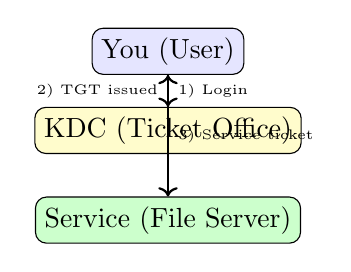
\begin{tikzpicture}[scale=0.67]
                    \node[draw, rounded corners, fill=blue!10] (user) at (0, 2.5) {You (User)};
                    \node[draw, rounded corners, fill=yellow!20] (kdc) at (0, 1.0) {KDC (Ticket Office)};
                    \node[draw, rounded corners, fill=green!20] (app) at (0, -0.7) {Service (File Server)};
                    \draw[->, thick] (user) -- (kdc) node[midway, right, font=\tiny] {1) Login};
                    \draw[->, thick] (kdc) -- (user) node[midway, left, font=\tiny] {2) TGT issued};
                    \draw[->, thick] (user) -- (app) node[midway, right, font=\tiny] {3) Service ticket};
                \end{tikzpicture}
            \end{center}
            \vspace{0.3em}
            \footnotesize
            Your password never travels to the file server. Only a short-lived ticket does. Less exposure means less risk.
        \end{column}
    \end{columns}
\end{frame}

\begin{frame}{Digital Certificates: Your Network ID Card}
    \begin{columns}[T]
        \begin{column}{0.48\textwidth}
            \footnotesize
            A \keyterm{digital certificate} is an electronic document that proves a server (or user) is who it claims to be.

            \vspace{0.3em}
            Think of it like a passport:
            \begin{itemize}
                \item It contains identity information (name, domain, public key).
                \item A trusted authority --- a \keyterm{Certificate Authority (CA)} --- has verified the identity and signed the certificate.
                \item Others trust it because they trust the issuer.
            \end{itemize}

            \vspace{0.3em}
            You encounter certificates constantly:
            \begin{itemize}
                \item The padlock in your browser = HTTPS certificate.
                \item VPN connections.
                \item Secure Wi-Fi (802.1X/EAP-TLS).
            \end{itemize}
        \end{column}
        \begin{column}{0.48\textwidth}
            \footnotesize
            \textbf{PKI} (Public Key Infrastructure) is the full system of CAs, certificates, and trust rules.

            \vspace{0.3em}
            \textbf{Chain of trust:}
            \begin{itemize}
                \item A \textbf{Root CA} is the ultimate trusted authority.
                \item \textbf{Intermediate CAs} sit below the Root CA and issue certificates to servers and users.
                \item Your browser ships with a built-in list of trusted Root CAs.
            \end{itemize}

            \begin{exampleblock}{Beginner checkpoint}
                \footnotesize
                If a site's certificate is expired, unsigned, or doesn't match the domain name, your browser shows a warning. That warning means the chain of trust is broken --- do not proceed.
            \end{exampleblock}
        \end{column}
    \end{columns}
\end{frame}

\begin{frame}{Key Management: Protecting the Keys to the Kingdom}
    \begin{columns}[T]
        \begin{column}{0.5\textwidth}
            \footnotesize
            Encryption is only as strong as the protection around the \textbf{keys} used to lock and unlock data. Having encryption and managing keys poorly is like locking your door and leaving the key under the mat.

            \vspace{0.3em}
            \begin{block}{Key Lifecycle}
                \footnotesize
                \begin{enumerate}
                    \item \textbf{Generate}: Create keys with strong randomness (entropy).
                    \item \textbf{Store}: Keep private keys in secure hardware vaults, not in code or configuration files.
                    \item \textbf{Rotate}: Replace keys on a regular schedule, or immediately after a suspected compromise.
                    \item \textbf{Revoke/Destroy}: Retire old keys completely --- no stale copies.
                \end{enumerate}
            \end{block}
        \end{column}
        \begin{column}{0.46\textwidth}
            \begin{alertblock}{Common Failures}
                \footnotesize
                \begin{itemize}
                    \item Hardcoded credentials or keys in source code (attackers search GitHub for these automatically).
                    \item One private key shared across many servers.
                    \item Long-lived keys that are never rotated.
                \end{itemize}
            \end{alertblock}
            \begin{exampleblock}{Revocation: CRL and OCSP}
                \footnotesize
                When a certificate is compromised, it is added to a \textbf{CRL} (Certificate Revocation List) or checked via \textbf{OCSP} (Online Certificate Status Protocol) so systems stop trusting it immediately.
            \end{exampleblock}
        \end{column}
    \end{columns}
\end{frame}

\begin{frame}{Federated Identity and SAML}
    \begin{columns}[T]
        \begin{column}{0.54\textwidth}
            \footnotesize
            \keyterm{Federated identity} lets one organization trust another organization's authentication. You log in with your home organization's credentials and get access to a partner's service --- no second account needed.

            \vspace{0.3em}
            \textbf{Real-world examples:} ``Log in with Google,'' ``Sign in with your university account'' on a third-party tool.

            \vspace{0.3em}
            \begin{block}{SAML in Plain Language}
                \footnotesize
                \textbf{SAML} (Security Assertion Markup Language) is the standard protocol that carries federated login information.
                \begin{itemize}
                    \item The \textbf{Identity Provider (IdP)}: your home org that knows who you are.
                    \item The \textbf{Service Provider (SP)}: the external site you want to use.
                    \item The IdP sends a signed, tamper-proof \textbf{assertion} to the SP: ``Yes, this is Alice; she works here and has these attributes.''
                \end{itemize}
            \end{block}
        \end{column}
        \begin{column}{0.42\textwidth}
            \begin{center}
                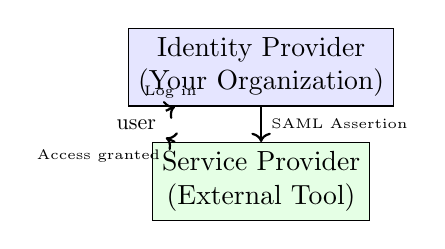
\begin{tikzpicture}[scale=0.66]
                    \node[draw, fill=blue!10, align=center] (idp) at (0, 2) {Identity Provider\\(Your Organization)};
                    \node[draw, fill=green!10, align=center] (sp) at (0, -0.2) {Service Provider\\(External Tool)};
                    \node (u) at (-2.4, 0.9) {\iconuser[0.5cm]};
                    \draw[->, thick] (u) -- (idp) node[midway, above, font=\tiny] {Log in};
                    \draw[->, thick] (idp) -- (sp) node[midway, right, font=\tiny] {SAML Assertion};
                    \draw[->, thick] (sp) -- (u) node[midway, below left, font=\tiny] {Access granted};
                \end{tikzpicture}
            \end{center}
            \vspace{0.2em}
            \footnotesize
            \textbf{Why it matters:} One account to manage, one place to deprovision when someone leaves.
        \end{column}
    \end{columns}
\end{frame}

\begin{frame}{Remote Authentication: RADIUS and TACACS+}
    \footnotesize
    When many users log into network devices or the corporate network from different locations, authentication needs to happen on a \emph{central server} --- not device-by-device. Two protocols handle this:

    \vspace{0.4em}
    \begin{columns}[T]
        \begin{column}{0.48\textwidth}
            \begin{block}{RADIUS}
                \footnotesize
                \textbf{Remote Authentication Dial-In User Service}
                \begin{itemize}
                    \item Common use: Wi-Fi login (802.1X), VPN, wired port authentication.
                    \item Combines authentication and authorization in a single response.
                    \item Uses UDP (connectionless, faster but less reliable transport).
                \end{itemize}
                \emph{Think: A fast ID check at the building entrance --- approve or deny, quickly.}
            \end{block}
        \end{column}
        \begin{column}{0.48\textwidth}
            \begin{block}{TACACS+}
                \footnotesize
                \textbf{Terminal Access Controller Access-Control System Plus}
                \begin{itemize}
                    \item Common use: admin logins to routers, switches, and firewalls.
                    \item Fully separates Authentication, Authorization, and Accounting.
                    \item Uses TCP (reliable) and encrypts the entire payload.
                    \item Can control which \emph{specific commands} each user is allowed to run.
                \end{itemize}
                \emph{Think: A detailed background check with a full activity log.}
            \end{block}
        \end{column}
    \end{columns}

    \vspace{0.3em}
    \begin{exampleblock}{Rule of thumb}
        \footnotesize
        Use RADIUS for endpoint and user access (Wi-Fi, VPN). Use TACACS+ for network device administration where command-level accountability matters.
    \end{exampleblock}
\end{frame}

\begin{frame}{Case Study: Cinderella's Co-Working Login Chaos}
    \begin{block}{Scenario}
        \scriptsize
        Cinderella manages a small startup from a co-working space. Her team uses three separate cloud (SaaS) tools: a CRM for client contacts, a source-code repository, and an invoicing app. Each tool has its own independent login system.

        A contractor's last day is Friday at 5~PM. Cinderella manually removes their account from the CRM. On Monday morning, finance discovers unauthorized invoice edits and a new vendor payout rule that nobody approved.

        Investigation reveals:
        \begin{itemize}\setlength{\itemsep}{1pt}
            \item The contractor's account was removed from the CRM but remained active in the invoicing app.
            \item Login records show access from a home IP address at 11:42~PM Sunday night.
        \end{itemize}
    \end{block}
    \scriptsize
    \textbf{Discussion Questions}
    \begin{enumerate}\setlength{\itemsep}{1pt}
        \item Which identity management flaw caused this? (What happens when offboarding is manual and spread across separate systems?)
        \item What single architectural change would have prevented the Sunday-night access?
        \item What logs would you need to determine the full scope of the damage?
    \end{enumerate}
\end{frame}

\begin{frame}{Case Study Solution: Cinderella's Co-Working Login Chaos}
    \begin{exampleblock}{Recommended Response}
        \footnotesize
        \begin{enumerate}
            \item \textbf{Root cause:} Separate identity stores with no central management. Manual offboarding missed one system. This is exactly the problem centralized identity (SSO) solves --- remove access in one place and it is gone everywhere.
            \item \textbf{Structural fix:} Centralized identity with automated deprovisioning. When the contractor is removed from the identity provider, all three tools lose access simultaneously. MFA would have made the Sunday-night login much harder even with valid credentials.
            \item \textbf{Containment:} Revoke all active sessions immediately, freeze invoice workflow changes, and revert unauthorized records.
            \item \textbf{Audit data:} Correlate login timestamps, session IDs, source IP addresses, and change records across all three tools to establish the complete impact timeline.
        \end{enumerate}
    \end{exampleblock}
    \begin{alertblock}{Key Principle}
        \footnotesize
        Identity controls are only as strong as your offboarding process. If offboarding is manual, it will eventually be incomplete. Automate it.
    \end{alertblock}
\end{frame}

% =============================================================================
\section{Authorization and Account Management}
\subsection{What You Can Do, and Who Watches}
% =============================================================================

\articleonly{
This section covers authorization models, privileged access management, directory services (LDAP and LDAPS), and account governance.
}

% --- NEW SLIDE ---
\begin{frame}{From Authentication to Authorization}
    \footnotesize
    Authentication answered the question: \emph{``Who are you?''}

    Authorization answers the next question: \emph{``Now that we know who you are --- what are you allowed to do?''}

    \vspace{0.5em}
    \begin{exampleblock}{A Hospital Analogy}
        \footnotesize
        A doctor and a janitor both badge in at the hospital entrance. Both \textbf{authenticated} successfully --- the system knows who they are. But the doctor can open patient records; the janitor cannot. The difference in what each person can \emph{do} is \textbf{authorization}.
    \end{exampleblock}

    \vspace{0.4em}
    \begin{alertblock}{The most common access mistake}
        \footnotesize
        Most security incidents involving insider access are not sophisticated attacks. They are \emph{permission mistakes}: someone had access they should never have had, and eventually it was abused --- or stolen by an outsider. Getting authorization right matters just as much as getting authentication right.
    \end{alertblock}
\end{frame}

\begin{frame}{Authorization and Role-Based Access Control (RBAC)}
    \footnotesize
    \keyterm{RBAC} (Role-Based Access Control) is the most common authorization model. Instead of assigning permissions to each individual person, you define \textbf{roles} and grant permissions to those roles.

    \vspace{0.4em}
    \begin{columns}[T]
        \begin{column}{0.5\textwidth}
            \begin{block}{How RBAC Works}
                \footnotesize
                \begin{enumerate}
                    \item Define job roles (Helpdesk, Network Admin, Security Analyst, Intern).
                    \item Map the \emph{minimum} permissions each role actually needs.
                    \item Assign users to roles, not to individual permissions.
                    \item When someone changes jobs, change their role --- not dozens of individual permissions.
                \end{enumerate}
            \end{block}
        \end{column}
        \begin{column}{0.46\textwidth}
            \begin{exampleblock}{Example Role Mapping}
                \footnotesize
                \begin{itemize}
                    \item \textbf{Helpdesk}: Reset passwords, create support tickets.
                    \item \textbf{Network Admin}: Configure switches and routers.
                    \item \textbf{Security Analyst}: Read logs only, no configuration rights.
                    \item \textbf{Intern}: Read-only access to training materials.
                \end{itemize}
            \end{exampleblock}
        \end{column}
    \end{columns}

    \vspace{0.3em}
    \begin{alertblock}{Least Privilege}
        \footnotesize
        \keyterm{Least privilege} means giving each user the minimum access needed to do their job --- and nothing more. Excess permissions are a hidden, silent risk sitting in your system waiting to be exploited.
    \end{alertblock}
\end{frame}

\begin{frame}{Privileged Access Management (PAM)}
    \begin{columns}[T]
        \begin{column}{0.52\textwidth}
            \footnotesize
            \keyterm{PAM} (Privileged Access Management) provides extra controls specifically for \textbf{admin-level accounts} --- the accounts that can change configurations, access everything, and cause the most damage if compromised.

            \vspace{0.4em}
            \textbf{Core PAM controls}
            \begin{itemize}
                \item \textbf{Vault credentials:} Store admin passwords in an encrypted vault, not in shared spreadsheets or sticky notes.
                \item \textbf{Just-in-time (JIT) elevation:} Grant admin rights only for a specific approved task, then remove them automatically.
                \item \textbf{Approval workflows:} High-risk actions require a supervisor to approve first.
                \item \textbf{Session recording:} Every privileged session is recorded for investigation and compliance.
            \end{itemize}
        \end{column}
        \begin{column}{0.44\textwidth}
            \footnotesize
            \textbf{Quick wins even without a PAM tool}
            \begin{itemize}
                \item Eliminate shared admin accounts --- every person needs their own named account.
                \item Never use your admin account for everyday tasks like email or web browsing.
                \item Log all privileged actions to a central, tamper-resistant syslog server.
            \end{itemize}

            \begin{exampleblock}{What ``good'' looks like}
                \footnotesize
                Admin rights are temporary, approved, recorded, and automatically expired. Nobody uses \texttt{root} or \texttt{Administrator} for daily work.
            \end{exampleblock}
        \end{column}
    \end{columns}
\end{frame}

\begin{frame}{LDAP: The Network's Phone Book}
    \begin{columns}[T]
        \begin{column}{0.5\textwidth}
            \footnotesize
            \keyterm{LDAP} (Lightweight Directory Access Protocol) is the standard protocol for looking up user accounts, group memberships, and identity attributes from a central directory --- like Microsoft Active Directory.

            \vspace{0.3em}
            Think of it as the network's \textbf{phone book}: when an application needs to know ``Is Alice in the Engineering group?'' it asks the directory server using LDAP, and the directory answers.

            \vspace{0.3em}
            \begin{itemize}
                \item Single, authoritative source for who exists and what groups they belong to.
                \item Applications use LDAP group membership to make authorization decisions.
                \item Supported across Linux, Windows, network devices, and cloud services.
            \end{itemize}
        \end{column}
        \begin{column}{0.46\textwidth}
            \begin{exampleblock}{Reading an LDAP Address (DN)}
                \footnotesize
                Every entry in the directory has a unique address called a \textbf{Distinguished Name (DN)}:

                \vspace{0.3em}
                \texttt{cn=alice,ou=engineering,dc=example,dc=edu}

                \vspace{0.3em}
                Reading right to left: the domain is \texttt{example.edu}, the organizational unit is \texttt{engineering}, and the user's common name (\texttt{cn}) is \texttt{alice}.
            \end{exampleblock}
            \begin{alertblock}{Operational note}
                \footnotesize
                If group memberships are wrong in LDAP, authorization will be wrong in every application that reads from it.
            \end{alertblock}
        \end{column}
    \end{columns}
\end{frame}

\begin{frame}{LDAPS: Encrypting the Phone Book}
    \begin{columns}[T]
        \begin{column}{0.48\textwidth}
            \footnotesize
            Plain \textbf{LDAP} (port 389) sends directory queries and credentials across the network in \emph{cleartext}. Anyone who can capture the traffic can read usernames, passwords, and group data.

            \vspace{0.4em}
            \keyterm{LDAPS} (LDAP Secure, port 636) wraps LDAP traffic in \textbf{TLS} encryption --- the same technology that makes HTTPS secure. Credentials and query results are protected in transit.

            \vspace{0.3em}
            \textbf{StartTLS} is an alternative approach: the connection starts as plain LDAP on port 389, then upgrades to encrypted mid-session before any credentials are sent.
        \end{column}
        \begin{column}{0.48\textwidth}
            \begin{alertblock}{LDAPS Hardening Checklist}
                \footnotesize
                \begin{itemize}
                    \item \textbf{Disable anonymous binds}: Do not let unauthenticated queries browse the directory.
                    \item \textbf{Enforce TLS 1.2 or higher}: Older TLS versions have known weaknesses.
                    \item \textbf{Restrict bind accounts}: The service account apps use to query LDAP should be read-only with minimal permissions.
                    \item \textbf{Log failed bind attempts}: Repeated failures may indicate a brute-force attack against directory credentials.
                \end{itemize}
            \end{alertblock}
        \end{column}
    \end{columns}
\end{frame}

\begin{frame}[fragile]{Example: Verifying a Secure LDAP Connection}
    \footnotesize
    On Linux, the \texttt{ldapsearch} command-line tool can test whether an LDAPS connection is working. A successful result confirms the encrypted connection is established and the server certificate is trusted.

    \vspace{0.4em}
    \begin{exampleblock}{Connecting securely on port 636 (LDAPS)}
        \scriptsize
\begin{verbatim}
$ ldapsearch -H ldaps://ad.example.com:636 \
             -D "cn=admin,dc=example,dc=com" -W
Enter LDAP Password:
# extended LDIF
# LDAPv3
# LDAP successful bind ...
\end{verbatim}
    \end{exampleblock}

    \begin{alertblock}{If the connection fails, check in order}
        \footnotesize
        1)~Is the server's TLS certificate valid and trusted by this client? \quad
        2)~Is port 636 open through the firewall? \quad
        3)~Is the directory server configured to accept LDAPS connections?
    \end{alertblock}
\end{frame}

\begin{frame}{Case Study: Little Red's Hospital Access Mix-Up}
    \begin{block}{Scenario}
        \footnotesize
        Little Red works at a hospital help desk. During her first week, she notices something alarming: interns starting their rotation can open both help desk ticketing tools \emph{and} the confidential payroll and HR compensation records.

        After checking the directory, she finds one broad LDAP group called \texttt{staff\_all} that grants access to everything simultaneously.

        Additional details:
        \begin{itemize}
            \item Two temporary interns were provisioned using the full-time employee account template, giving them far more access than their role requires.
            \item A shared account named ``HRAdmin'' was used during weekend support shifts --- no one knows exactly who used it or when.
            \item There is no approval record or audit trail for payroll export actions taken over the past six months.
        \end{itemize}
    \end{block}
    \textbf{Discussion Questions}
    \begin{enumerate}
        \item Which principles failed: least privilege, separation of duties, or both? Explain.
        \item How should the LDAP group structure be redesigned?
        \item What PAM controls should be added for payroll and HR admin functions?
    \end{enumerate}
\end{frame}

\begin{frame}{Case Study Solution: Little Red's Hospital Access Mix-Up}
    \begin{exampleblock}{Recommended Response}
        \footnotesize
        \begin{enumerate}
            \item \textbf{Both principles failed.} Interns had access far beyond their job scope (\emph{least privilege} violation). The same account could perform both help desk and payroll functions (\emph{separation of duties} violation). The shared HRAdmin account makes individual accountability impossible.
            \item \textbf{Directory redesign:} Replace \texttt{staff\_all} with purpose-specific groups: \texttt{intern\_readonly}, \texttt{helpdesk}, \texttt{hr\_analyst}, \texttt{payroll\_admin}. Each group maps to only the minimum permissions that role actually requires.
            \item \textbf{PAM controls:} Eliminate the shared HRAdmin account; require individual named accounts for all HR work. Add just-in-time elevation with manager approval for payroll exports. Record all privileged HR sessions.
            \item \textbf{Governance:} Implement quarterly access reviews where managers certify which users still need each sensitive permission.
        \end{enumerate}
    \end{exampleblock}
\end{frame}

% =============================================================================
\section{Network Hardening}
\subsection{Reducing the Attack Surface}
% =============================================================================

\articleonly{
This section covers defense-in-depth principles, device and service hardening, and reducing attack surface through disciplined configuration.
}

% --- NEW SLIDE ---
\begin{frame}{What Does ``Hardening'' Actually Mean?}
    \footnotesize
    \keyterm{Hardening} means configuring a device or system to remove unnecessary features, close unused access points, and replace insecure defaults that attackers already know about.

    \vspace{0.4em}
    \begin{exampleblock}{The New Router Analogy}
        \footnotesize
        A brand-new home router ships from the factory with:
        \begin{itemize}
            \item Username: \texttt{admin} \quad Password: \texttt{admin}
            \item Remote management enabled from the internet
            \item Firmware with known, publicly documented vulnerabilities
        \end{itemize}
        Millions of routers ship with \emph{identical} default credentials. Attackers automate internet-wide scans for them within days of a new model's release.

        \vspace{0.2em}
        \textbf{Hardening} that router: change the admin password, disable internet-facing remote management, and update the firmware. You go from ``default target'' to ``not worth the effort.''
    \end{exampleblock}

    \begin{alertblock}{Rule of thumb}
        \footnotesize
        If a feature or service is not actively being used, disable it. Every unused service is an open door you may have forgotten.
    \end{alertblock}
\end{frame}

\begin{frame}{Defense in Depth: No Single Control Is Enough}
    \footnotesize
    \keyterm{Defense in depth} means building multiple independent layers of security so that bypassing one control does not result in complete compromise.

    \vspace{0.2em}
    \begin{center}
        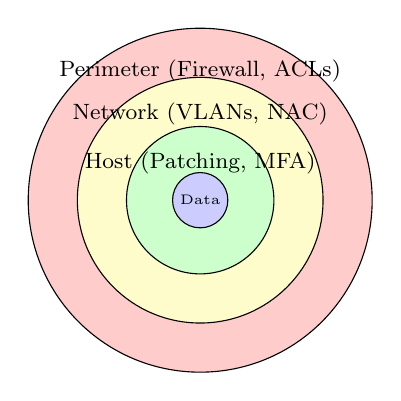
\begin{tikzpicture}[scale=0.78]
            \draw[fill=red!20] (0,0) circle (2.8cm);
            \node at (0, 2.1) {\footnotesize Perimeter (Firewall, ACLs)};
            \draw[fill=yellow!20] (0,0) circle (2.0cm);
            \node at (0, 1.4) {\footnotesize Network (VLANs, NAC)};
            \draw[fill=green!20] (0,0) circle (1.2cm);
            \node at (0, 0.6) {\footnotesize Host (Patching, MFA)};
            \draw[fill=blue!20] (0,0) circle (0.45cm);
            \node[font=\tiny] at (0, 0) {Data};
        \end{tikzpicture}
    \end{center}
    \footnotesize
    An attacker who bypasses the firewall still faces VLANs, host hardening, and encryption around the data itself.

    \vspace{0.2em}
    \textbf{Common beginner mistake:} Trusting only the firewall and neglecting identity controls, patching, and monitoring.
\end{frame}

\begin{frame}{Layered Hardening: A Small Office Example}
    \footnotesize
    Defense in depth does not require expensive tools. A small office can layer simple, affordable controls effectively.

    \vspace{0.4em}
    \begin{table}[]
        \renewcommand{\arraystretch}{1.2}
        \centering
        \begin{tabular}{|l|l|l|}
        \hline
        \rowcolor[HTML]{EFEFEF} \textbf{Layer} & \textbf{Concrete Control} & \textbf{What It Prevents} \\ \hline
        Identity & MFA for all remote logins & Stolen passwords used to log in remotely \\ \hline
        Network & VLANs separating guest from staff & Guest devices reaching internal file servers \\ \hline
        Host & Automatic patching + local firewall & Known exploits and exposed local services \\ \hline
        Physical & Lock server closet, disable unused ports & Someone plugging in a rogue device \\ \hline
        Monitoring & Central syslog and email alerts & Attacks that slip through other layers \\ \hline
        \end{tabular}
    \end{table}

    \begin{exampleblock}{Key insight}
        \footnotesize
        When one layer fails, the remaining layers slow the attacker down, buy time for detection, and create an audit trail that supports incident response.
    \end{exampleblock}
\end{frame}

\begin{frame}{Device and Service Hardening: The Checklist}
    \begin{columns}[T]
        \begin{column}{0.49\textwidth}
            \footnotesize
            \textbf{Device hardening steps}
            \begin{enumerate}
                \item Change all default credentials immediately on first login.
                \item Disable interfaces, ports, and management services that are not in use.
                \item Restrict management access: only allow SSH connections from specific trusted admin IP addresses.
                \item Apply firmware and security patches on a regular, documented schedule.
                \item Use encrypted management protocols only:
                    SSH instead of Telnet, HTTPS instead of HTTP.
            \end{enumerate}
        \end{column}
        \begin{column}{0.49\textwidth}
            \footnotesize
            \textbf{Service hardening}
            \begin{itemize}
                \item Remove or disable any service not actively needed (every running process is a potential target).
                \item Replace insecure protocols with secure equivalents:
                    \begin{itemize}\footnotesize
                        \item Telnet \textrightarrow\ SSH
                        \item FTP \textrightarrow\ SFTP
                        \item HTTP \textrightarrow\ HTTPS
                        \item SNMPv1/v2c \textrightarrow\ SNMPv3
                    \end{itemize}
                \item Enable host-based firewalls on servers.
                \item Send all service logs to a central, tamper-resistant syslog server.
            \end{itemize}
        \end{column}
    \end{columns}
\end{frame}

% =============================================================================
\section{Switch Security}
\subsection{Controlling Who Gets On the Network}
% =============================================================================

\articleonly{
This section covers switch-level enforcement controls: port security, 802.1X authentication, Layer 2 guard features, and port mirroring for traffic visibility.
}

\begin{frame}{Network Access Control (NAC) and Port Security}
    \begin{columns}[T]
        \begin{column}{0.5\textwidth}
            \footnotesize
            \keyterm{Network Access Control (NAC)} means the network itself verifies whether a device is permitted before granting full access.

            \vspace{0.3em}
            Think of an airport: you do not walk straight to the gate. You clear a security checkpoint first. NAC is that checkpoint for your network ports.

            \vspace{0.3em}
            \textbf{Port security} is a simpler, switch-level form of this: limit which devices --- identified by their \textbf{MAC address} (the hardware ID burned into every network interface) --- can connect to each port.

            \begin{itemize}
                \item Set a maximum of 1--2 MAC addresses per access port.
                \item \textbf{Sticky learning}: the switch remembers the first device it sees.
                \item Violation actions: \textbf{protect} (drop silently), \textbf{restrict} (drop and log), or \textbf{shutdown} (disable the port entirely).
            \end{itemize}
        \end{column}
        \begin{column}{0.46\textwidth}
            \footnotesize
            \textbf{Why this matters}
            \begin{itemize}
                \item Prevents someone from plugging an unauthorized device into a wall jack.
                \item Stops a visitor from adding an unmanaged hub or mini-switch to multiply access.
            \end{itemize}

            \vspace{0.4em}
            \textbf{Basic design pattern:}
            \begin{enumerate}
                \item Authenticate the device or user.
                \item Assign to the correct VLAN based on identity.
                \item Monitor port activity continuously.
            \end{enumerate}

            \begin{exampleblock}{Design tip}
                \footnotesize
                Build a secure template for access ports. Every new port is locked down by default, not open by default.
            \end{exampleblock}
        \end{column}
    \end{columns}
\end{frame}

\begin{frame}[fragile]{Example: Port Security on a Lobby Switch}
    \footnotesize
    This Cisco switch configuration restricts a lobby port to exactly one device. The switch learns and remembers the first MAC address it sees (``sticky''), and shuts the port if anything else connects.

    \vspace{0.4em}
    \begin{exampleblock}{Cisco IOS port security configuration}
        \scriptsize
\begin{verbatim}
interface GigabitEthernet1/0/2
 switchport mode access
 switchport port-security
 switchport port-security maximum 1
 switchport port-security mac-address sticky
 switchport port-security violation shutdown
\end{verbatim}
    \end{exampleblock}

    \begin{alertblock}{What happens when a second device connects?}
        \scriptsize
\begin{verbatim}
%PORT_SECURITY-2-PSECURE_VIOLATION: Security violation occurred,
port Gi1/0/2 is shutting down.
\end{verbatim}
    \end{alertblock}

    \footnotesize
    The port disables itself and requires manual administrator recovery. One wall jack, one expected device, one known MAC address.
\end{frame}

% --- NEW SLIDE ---
\begin{frame}{What is IEEE 802.1X? The Velvet Rope at the Network Door}
    \footnotesize
    \keyterm{802.1X} is a standard that controls access to a network port or Wi-Fi connection at the \emph{identity} level --- not just the device level.

    \vspace{0.3em}
    \begin{exampleblock}{Analogy: The Nightclub Velvet Rope}
        \footnotesize
        A bouncer does not let anyone through just because they walked up. They check your ID and verify you are on the list. With 802.1X, your laptop may be physically plugged into a switch port --- but \emph{no network traffic flows} until you have successfully authenticated. The port is the velvet rope.
    \end{exampleblock}

    \vspace{0.3em}
    \begin{columns}[T]
        \begin{column}{0.32\textwidth}
            \begin{block}{Supplicant}
                \footnotesize
                Your laptop or phone --- the device \emph{requesting} network access.
            \end{block}
        \end{column}
        \begin{column}{0.32\textwidth}
            \begin{block}{Authenticator}
                \footnotesize
                The switch or Wi-Fi access point that \emph{enforces} the check. It holds traffic until authentication succeeds.
            \end{block}
        \end{column}
        \begin{column}{0.32\textwidth}
            \begin{block}{Auth Server}
                \footnotesize
                Usually a RADIUS server that \emph{validates} the credentials and tells the switch: permit or deny.
            \end{block}
        \end{column}
    \end{columns}

    \vspace{0.3em}
    \footnotesize
    \textbf{EAP} (Extensible Authentication Protocol) is the ``conversation format'' used between these three parties. Common methods: \textbf{EAP-TLS} (certificate-based, strongest phishing resistance) and \textbf{PEAP} (username/password inside an encrypted tunnel).
\end{frame}

\begin{frame}{Port Guards: Stopping Layer 2 Attacks}
    \footnotesize
    Layer 2 (the switch layer) has specific vulnerabilities. Guard features are built into managed switches to block them.

    \vspace{0.3em}
    \begin{columns}[T]
        \begin{column}{0.5\textwidth}
            \begin{block}{Guard Features Explained}
                \footnotesize
                \begin{itemize}
                    \item \textbf{BPDU Guard}: \textbf{BPDUs} (Bridge Protocol Data Units) are control messages switches exchange to manage spanning tree topology. Only switches should send them. BPDU Guard shuts a port the moment BPDUs arrive from a device that should not be sending them --- like a rogue switch someone plugged in.
                    \item \textbf{Root Guard}: Prevents any device from claiming to be the ``root bridge'' (the master reference switch), which would disrupt the entire switching topology.
                    \item \textbf{DHCP Snooping}: Blocks unauthorized DHCP servers from handing out fake IP addresses and gateway settings.
                    \item \textbf{DAI} (Dynamic ARP Inspection): Validates ARP packets against a trusted binding table to prevent ARP spoofing, where an attacker redirects traffic through their device.
                \end{itemize}
            \end{block}
        \end{column}
        \begin{column}{0.46\textwidth}
            \begin{alertblock}{Why This Matters}
                \footnotesize
                Without these guards, a single rogue device plugged into a wall jack can:
                \begin{itemize}
                    \item Intercept and read all traffic on the segment (man-in-the-middle).
                    \item Hand out fake IP settings, making the network unreachable.
                    \item Disrupt spanning tree and bring down switching for the entire floor.
                \end{itemize}
            \end{alertblock}
            \vspace{0.2em}
            \footnotesize
            Apply these guards to all access ports. Explicitly exclude trunk and uplink ports (which legitimately carry BPDUs and multiple VLANs).
        \end{column}
    \end{columns}
\end{frame}

\begin{frame}[fragile]{Example: Recovering from a Port Violation}
    \footnotesize
    When BPDU Guard or port security triggers, the switch places the port in \texttt{err-disabled} state. Nothing can use the port until an administrator manually recovers it --- which is intentional.

    \vspace{0.4em}
    \begin{exampleblock}{What you see on the console}
        \scriptsize
\begin{verbatim}
%PM-4-ERR_DISABLE: psecure-mac-violation error detected on Gi1/0/2,
putting Gi1/0/2 in err-disable state

Switch# show interfaces status err-disabled
Port      Name              Status        Reason
Gi1/0/2   Lobby_Printer     err-disabled  psecure-mac-violation
\end{verbatim}
    \end{exampleblock}

    \begin{block}{Recovery steps}
        \footnotesize
        \begin{enumerate}
            \item Physically remove the unauthorized device from the port.
            \item Enter interface configuration: \texttt{interface GigabitEthernet1/0/2}
            \item Run \texttt{shutdown} then \texttt{no shutdown} to reset the port state.
            \item Confirm recovery: \texttt{show interfaces GigabitEthernet1/0/2 status}
        \end{enumerate}
    \end{block}
\end{frame}

\begin{frame}{Port Mirroring (SPAN): Watching Without Touching}
    \begin{columns}[T]
        \begin{column}{0.52\textwidth}
            \footnotesize
            \keyterm{Port mirroring} (also called \textbf{SPAN} --- Switched Port ANalyzer) copies traffic from one or more switch ports to a dedicated monitor port. A security or analysis tool connected to that monitor port can see all the traffic without being in the path of that traffic.

            \vspace{0.3em}
            \begin{exampleblock}{Use Cases}
                \footnotesize
                \begin{itemize}
                    \item Security investigation: capture and replay suspicious traffic for analysis.
                    \item \textbf{IDS} (Intrusion Detection System) placement: the IDS watches all traffic and raises alerts without slowing down real traffic.
                    \item Performance troubleshooting: a packet analyzer watches live traffic to diagnose slowdowns.
                \end{itemize}
            \end{exampleblock}
        \end{column}
        \begin{column}{0.44\textwidth}
            \begin{alertblock}{Caution}
                \footnotesize
                Mirrored traffic contains \emph{everything} --- passwords, personal data, confidential files, health records. Treat the monitor port and capture device as high-security assets.
            \end{alertblock}
            \vspace{0.3em}
            \footnotesize
            \textbf{Best practice:} Mirror only the specific ports or VLANs relevant to your investigation. Mirroring everything creates excessive data and can overwhelm both analysis tools and storage.
        \end{column}
    \end{columns}
\end{frame}

\begin{frame}{Case Study: Jack and the Beanstalk Data Center}
    \begin{block}{Scenario}
        \footnotesize
        Jack's cloud startup rents space on a shared data center floor with contractor access during business hours. During a maintenance window, a visiting contractor plugs a small unmanaged switch (a ``mini-switch'') into an open wall port to get extra network ports for their equipment --- without asking anyone.

        Within the next hour:
        \begin{itemize}
            \item Nearby servers begin receiving incorrect default gateway addresses.
            \item VoIP phones start dropping calls and flapping between VLANs.
            \item Network monitoring shows unexpected BPDU traffic and multiple unauthorized DHCP offer packets originating from an access port.
        \end{itemize}
    \end{block}
    \textbf{Discussion Questions}
    \begin{enumerate}
        \item Which switch security controls would have blocked this before it started?
        \item Which guard features should be enabled on all access ports in this environment, and why?
        \item How could port mirroring help confirm exactly what the mini-switch was doing?
    \end{enumerate}
\end{frame}

\begin{frame}{Case Study Solution: Jack and the Beanstalk Data Center}
    \begin{exampleblock}{Recommended Response}
        \footnotesize
        \begin{enumerate}
            \item \textbf{Prevention:} 802.1X authentication would have blocked the unauthenticated mini-switch from gaining any network access at all. Port security with a MAC limit of 1 would have shut the port the moment a second device appeared behind it.
            \item \textbf{Guard features:} DHCP Snooping blocks the rogue DHCP server on the mini-switch. BPDU Guard shuts the port the moment spanning-tree BPDUs arrive from a non-switch device. DAI prevents any ARP spoofing the mini-switch might attempt to intercept traffic.
            \item \textbf{SPAN:} Mirror the affected access port to a capture device. Analyze the PCAP to confirm rogue DHCP offers, BPDU floods, and any ARP manipulation --- then document timestamps and affected endpoints for the incident report.
            \item \textbf{Operational fix:} Disable and label all unused ports. Contractor access to specific authorized ports only, documented in the change management system.
        \end{enumerate}
    \end{exampleblock}
\end{frame}

% =============================================================================
\section{Network Security Rules}
\subsection{ACLs, Proxies, and Filtering}
% =============================================================================

\articleonly{
This section covers Access Control Lists, proxy architectures, content filtering, and troubleshooting misconfigured rule sets.
}

\begin{frame}{Access Control Lists (ACLs): Traffic Rules for the Network}
    \begin{columns}[T]
        \begin{column}{0.5\textwidth}
            \footnotesize
            An \keyterm{ACL} (Access Control List) is an ordered list of rules on a router or firewall that decides whether to \textbf{permit} or \textbf{deny} each packet.

            \vspace{0.4em}
            \textbf{Three rules to understand first:}
            \begin{itemize}
                \item Rules are checked \textbf{top to bottom}. The \textbf{first matching rule wins} --- checking stops immediately.
                \item At the end of every ACL there is an \textbf{implicit deny all}. If no rule matches, the packet is dropped silently.
                \item \textbf{Standard ACLs} filter by source IP address only. \textbf{Extended ACLs} can filter by source, destination, protocol, and port number.
            \end{itemize}
        \end{column}
        \begin{column}{0.46\textwidth}
            \footnotesize
            \textbf{Think of it as a checklist at a border crossing:}
            \begin{enumerate}
                \item Where did this packet come from?
                \item Where is it going?
                \item What protocol and port is it using?
                \item Does the first matching rule say permit or deny?
                \item No match = implicit deny. Packet dropped.
            \end{enumerate}

            \begin{alertblock}{Most common beginner mistake}
                \footnotesize
                A broad \texttt{permit ip any any} rule near the top of the list quietly cancels every specific deny rule below it --- because the broad rule matches everything first.
            \end{alertblock}
        \end{column}
    \end{columns}
\end{frame}

\begin{frame}[fragile]{Example: Reading a Cisco ACL}
    \footnotesize
    Read this ACL line by line. It is applied to a guest Wi-Fi segment to control what guests can reach.

    \begin{exampleblock}{Cisco IOS Extended ACL --- GUEST\_RESTRICTION}
        \scriptsize
\begin{verbatim}
ip access-list extended GUEST_RESTRICTION
 10 permit udp any any eq 53       ! Allow DNS (port 53) -- guests need name lookups
 20 permit tcp any any eq 80       ! Allow HTTP (port 80)
 30 permit tcp any any eq 443      ! Allow HTTPS (port 443)
 40 deny ip any 10.0.0.0 0.255.255.255  ! Block internal network (10.x.x.x)
 50 permit ip any any              ! Allow all other internet traffic
\end{verbatim}
    \end{exampleblock}

    \begin{alertblock}{Why order matters critically}
        \footnotesize
        If lines 40 and 50 were swapped, line 50 (\texttt{permit ip any any}) would match \emph{every} packet first --- including traffic destined for the internal \texttt{10.0.0.0} network. Line 40 would never be evaluated. Guests could reach internal servers.
    \end{alertblock}
\end{frame}

\begin{frame}{Proxy Servers: The Helpful Middleman}
    \begin{columns}[T]
        \begin{column}{0.48\textwidth}
            \footnotesize
            A \keyterm{proxy server} sits between users and the internet (or between the internet and your servers). All traffic is routed through the proxy, where it can be inspected, filtered, logged, and controlled before reaching its destination.

            \vspace{0.4em}
            \textbf{Why use a proxy?}
            \begin{itemize}
                \item Require authentication before any internet access is granted.
                \item Block malicious or policy-violating websites.
                \item Cache frequently accessed content (faster for users, cheaper on bandwidth).
                \item Maintain a complete log of every URL users visit.
                \item Scan downloads for malware before they reach the endpoint.
            \end{itemize}
        \end{column}
        \begin{column}{0.48\textwidth}
            \begin{exampleblock}{Three Proxy Types}
                \footnotesize
                \begin{itemize}
                    \item \textbf{Forward proxy}: Internal users go \emph{out} through the proxy to the internet. The proxy protects and monitors your users.
                    \item \textbf{Reverse proxy}: External visitors come \emph{in} through the proxy to reach your servers. The proxy protects your servers and can load-balance across them.
                    \item \textbf{Transparent proxy}: Intercepts traffic automatically with no configuration required on user devices --- users may not know it exists.
                \end{itemize}
            \end{exampleblock}
        \end{column}
    \end{columns}
\end{frame}

\begin{frame}{Forward Proxy vs.\ Reverse Proxy}
    \footnotesize
    \begin{table}[]
        \renewcommand{\arraystretch}{1.3}
        \centering
        \begin{tabular}{|l|l|l|}
        \hline
        \rowcolor[HTML]{EFEFEF}
        \textbf{Feature} & \textbf{Forward Proxy} & \textbf{Reverse Proxy} \\ \hline
        Traffic direction & Outbound (users to internet) & Inbound (internet to your servers) \\ \hline
        Protects & Internal users & Internal servers \\ \hline
        Typical jobs & URL filtering, malware scan, caching & Load balance, WAF, TLS termination \\ \hline
        Does client know? & Usually (configured on device) & No (transparent to outside visitors) \\ \hline
        Example & Corporate web filter & nginx in front of a web application \\ \hline
        \end{tabular}
    \end{table}

    \vspace{0.3em}
    \begin{exampleblock}{Snow White's Studio}
        \footnotesize
        Snow White's editors browse the internet through a \textbf{forward proxy} that blocks malware-hosting domains. External clients previewing completed videos hit a \textbf{reverse proxy} that distributes load across render servers and hides their real addresses.
    \end{exampleblock}
\end{frame}

\begin{frame}{Content Filtering: More Than Blocking Websites}
    \begin{columns}[T]
        \begin{column}{0.5\textwidth}
            \footnotesize
            \keyterm{Content filtering} enforces organizational policy about what users can access, what files can be downloaded, and which domains can be contacted.

            \begin{block}{What Content Filtering Can Do}
                \footnotesize
                \begin{itemize}
                    \item \textbf{URL category blocking}: Block categories such as gambling, malware-hosting, or social media during work hours.
                    \item \textbf{DNS filtering}: Block known malicious domains before a TCP connection is even established.
                    \item \textbf{File type control}: Block executable files (\texttt{.exe}, \texttt{.ps1}) downloaded from unknown sources.
                    \item \textbf{Malware scanning}: Inspect downloaded files before they reach the user's device.
                    \item \textbf{Safe search enforcement}: Force safe-search mode on major search engines.
                \end{itemize}
            \end{block}
        \end{column}
        \begin{column}{0.46\textwidth}
            \begin{alertblock}{Balance Security and Usability}
                \footnotesize
                Overly aggressive filtering breaks legitimate business tools. A security researcher may need to visit sites that a ``hacking tools'' category would block. Work with users, not against them.
            \end{alertblock}
            \begin{exampleblock}{Deployment best practice}
                \footnotesize
                Start in \textbf{monitor-only mode}: log what \emph{would} be blocked without actually blocking it. Review logs for two weeks to identify false positives, then switch to enforcement.
            \end{exampleblock}
        \end{column}
    \end{columns}
\end{frame}

\begin{frame}{Misconfigured Firewalls and ACLs: How Rules Go Wrong}
    \begin{columns}[T]
        \begin{column}{0.48\textwidth}
            \begin{block}{Common Misconfigurations}
                \footnotesize
                \begin{itemize}
                    \item \textbf{Shadowed rules}: A broad rule earlier in the list matches all the traffic that a specific rule below it was meant to catch. The specific rule is ``shadowed'' and never runs.
                    \item \textbf{Any-any permit in production}: A catch-all allow rule left over from initial testing that was never removed.
                    \item \textbf{Wrong rule order}: Deny rules placed below the permit rules they were meant to override.
                    \item \textbf{Missing egress filtering}: Outbound traffic from your network is not filtered --- data exfiltration has no obstacle.
                \end{itemize}
            \end{block}
            \vspace{0.2em}
            \footnotesize
            Most ACL-related outages trace to rule \emph{order} mistakes, not missing rules.
        \end{column}
        \begin{column}{0.48\textwidth}
            \begin{alertblock}{Troubleshooting Approach}
                \footnotesize
                \begin{enumerate}
                    \item Write down the intended traffic matrix \emph{first}: what should be allowed, from where, to where.
                    \item Trace the packet path and identify every firewall or ACL it crosses.
                    \item Check hit counters --- a rule with zero hits is likely shadowed or unreachable.
                    \item Make the minimum change needed and retest before moving to the next change.
                \end{enumerate}
            \end{alertblock}
            \vspace{0.2em}
            \footnotesize
            Always have a tested rollback plan ready before applying changes in production.
        \end{column}
    \end{columns}
\end{frame}

\begin{frame}{Case Study: Snow White's Streaming Studio Firewall Meltdown}
    \begin{block}{Scenario}
        \footnotesize
        Snow White runs a media startup with seven remote editors and an on-premises render cluster. After a weekend firewall change, editors cannot sync project files or push final exports to the render cluster. General web browsing and social media still work fine.

        A review of the firewall ruleset reveals:
        \begin{itemize}
            \item A broad \texttt{permit ip any any} rule is positioned near the top of the list.
            \item A new deny rule targeting the file-sync service's ports is placed \emph{below} a general internet-allow rule.
            \item The change ticket has no documentation of which business traffic flows the change was intended to protect or affect.
        \end{itemize}
    \end{block}
    \textbf{Discussion Questions}
    \begin{enumerate}
        \item What ACL or firewall ordering problem is most likely responsible for the editors' issues?
        \item Which traffic flows should be explicitly permitted first in a corrected rule set?
        \item Where should content filtering be introduced to reduce risk without breaking editor workflows?
    \end{enumerate}
\end{frame}

\begin{frame}{Case Study Solution: Snow White's Streaming Studio Firewall Meltdown}
    \begin{exampleblock}{Recommended Response}
        \footnotesize
        \begin{enumerate}
            \item \textbf{Shadowed deny rule.} The \texttt{permit ip any any} rule above the file-sync deny matches all packets first, so the deny is never reached. The sync service traffic is being permitted by the broad rule, but something else in the path (possibly a different ACL or routing issue) is blocking it. Audit every policy enforcement point in the editor-to-render path.
            \item \textbf{Rule rebuild from a traffic matrix:} Explicitly permit editor-to-render traffic (specific source subnets, destination IPs, required ports). Permit sync service traffic by protocol and port. Place all specific permits \emph{before} any broad denies. Remove the any-any permit.
            \item \textbf{Content filtering:} Route general internet browsing through an authenticated forward proxy with URL category filtering. Keep render cluster and sync traffic on a separate, unfiltered path. Document the distinction in the change ticket.
        \end{enumerate}
    \end{exampleblock}
    \begin{alertblock}{Process lesson}
        \footnotesize
        No firewall change should go into production without a traffic matrix and a rollback plan documented in the change ticket.
    \end{alertblock}
\end{frame}

% =============================================================================
\section*{Module Summary}
% =============================================================================

\begin{frame}[t,allowframebreaks]{Module 10 Summary}
    \small
    \begin{itemize}
        \item \keyterm{AAA} (Authentication, Authorization, Accounting) is the framework behind every secure login: prove identity, apply permissions, log all activity.
        \item \keyterm{MFA} (Multi-Factor Authentication) combines independent factors to make stolen passwords insufficient on their own. Hardware keys and passkeys provide the strongest phishing resistance.
        \item \keyterm{SSO} and \keyterm{Kerberos} let users authenticate once and access many services via temporary tickets. \keyterm{SAML} extends this trust across organizational boundaries (federated identity).
        \item \keyterm{PKI} and digital certificates establish a chain of trust for encrypted communications. Key lifecycle management --- generate, store, rotate, revoke --- is as important as the encryption itself.
        \item \keyterm{RADIUS} handles endpoint and user access (Wi-Fi, VPN). \keyterm{TACACS+} handles network device administration with full command-level control and separation of AAA functions.
        \item \keyterm{RBAC} and least privilege minimize the blast radius of any compromised account. \keyterm{PAM} adds vaulting, just-in-time elevation, and session recording specifically for high-risk admin credentials.
        \item \keyterm{LDAP} centralizes identity lookups. \keyterm{LDAPS} encrypts that traffic in transit and should replace plain LDAP in all production environments.
        \item \keyterm{Hardening} removes default credentials, disables unused services, and closes unnecessary access paths before attackers can exploit them.
        \item Switch controls --- 802.1X, port security, DHCP Snooping, BPDU Guard, and DAI --- defend the access layer from both physical and Layer 2 attacks. Port mirroring (SPAN) enables visibility without inline risk.
        \item \keyterm{ACLs} enforce traffic policy on routers and firewalls; rule order is critical and an implicit deny applies to all unmatched traffic. Proxies and content filters extend policy enforcement to the application layer.
    \end{itemize}
\end{frame}

\articleonly{
\subsection*{Conclusion}
This module connected identity concepts to practical enforcement mechanisms: the AAA framework, authentication factors and MFA, SSO and Kerberos, digital certificates and PKI, remote authentication protocols, authorization governance via RBAC and PAM, directory services, host and switch hardening, and policy-driven traffic controls with ACLs and proxies. Each case study traced a real-world incident back to a failure in identity management, access control, or rule configuration --- and showed how good design prevents them.
}

\begin{frame}{Questions?}
    \begin{center}
        \begin{tikzpicture}[scale=1.4]
            \node (shield) at (0,0) {\faIcon{user-shield}};
            \node[above=0.5cm of shield, font=\Large\bfseries, text=rctcblue] {Identity + Hardening Complete};
            \node[below=0.5cm of shield, font=\small] {Any questions?};
        \end{tikzpicture}
    \end{center}
\end{frame}

\end{document}
